
\begin{figure}[h!]
    \centering
    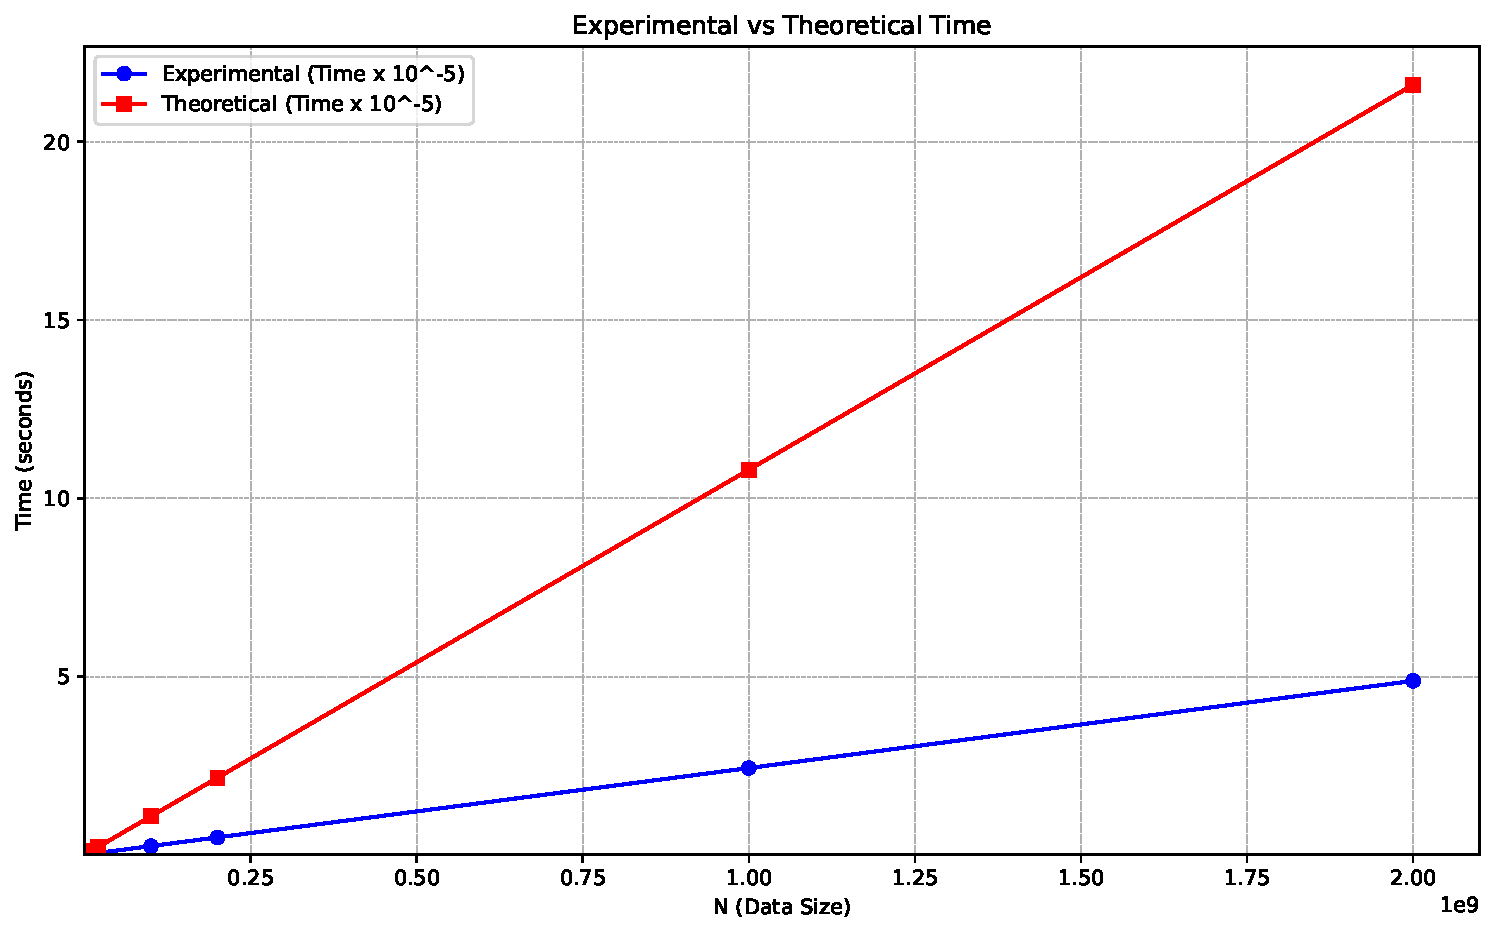
\includegraphics[width=0.85\textwidth]{Questions/Part2/plot.pdf}
    \label{fig:time_plot}
\end{figure}

\vspace{1cm}

\begin{prettyBox}{Conclusion}{green}
From the two plots we can conclude that the theoritical complexity plot is similar to the experimental complexity plot,
and also that theoritcal complexity follows a pattern in values since its \(\Delta t\) has a static value
\end{prettyBox}

\newpage 

To Draw the plots i used the below python script :

\vspace{1cm}

\lstinputlisting[style=pythonstyle2,inputencoding=utf8]{Questions/Part2/draw.py}
